\pattern{Event Based}
\begin{summary}
Event-based architecture is an architecture style that uses the production and
consumption of events to control the behaviour of components. Instead of
components communicate directly by referencing or method call, they communicate
by sending and receiving events asynchronously.

There are two types of components call event producer and event consumer. Event
producer is a component that produces and sends event. It should maintain its
internal state and produce an event when some predefined state change happened.
Event  consumer is a component that receives and consumers event. It should
consumer the event that it receives and starts its process with respect to the
event. One component can be both event producer and consumer interchangeably in
the context of entire architecture by both producing and consuming events.
There is only one type of connector in this architecture called event bus.
Event bus is the medium on which the events are being transmitted.

Event-based architectures can simplify software design, development, and
testing because they minimize the connections between the components. Instead
of each component directly communicate to each other with high coupling and
complicated structure, they all communicate through the event bus which makes
communication elegant. Each component can be developed and tested independently
because they do not require to know other components. This can be very
beneficial to large projects since the complexity of the project grows linearly
instead of exponential.

Most applicable to specific kinds of problems \begin{itemize}[noitemsep]
    \item User interface: website browser
    \item Distributed application
\end{itemize}

\end{summary}

\comparison{\begin{itemize}
        \item Engender specific kinds of change resilience: 
● For removing an event bus and creating producers before creating an event
bus, we need to change producers to handle the invalid event bus because
producers might not be able to fire an event to an empty place/address
● For changing an event type for a typed event bus, we also need to maintain
consistency for producers and consumers as well. 
\end{itemize}
}{\begin{itemize}
        \item The event bus may become a bottleneck.
○ When there are too many producers are sending the message concurrently.
Therefore, the number of messages is larger than the number of events which the
event bus handled.
● Not sending message efficiency.
○ The event bus has the queue for event sending or receive. It can not send or
receive the message immediately. 
\end{itemize}}

\begin{nfps}
\item[Scalability] The Space decoupling
■ The event producers and event consumers do not need to know each other.
■ The event producers do not hold references to event consumers or know how many of them are interacting and vice versa.
○ The time decoupling
■ The event producers and event consumers do not need to be actively involved in the interaction at the same time.
○ The synchronization decoupling
■ The event producers are not blocked while producing events and they can receive events.
■ The event consumers can get the notification when an event happens while performing some other concurrent activity.
● Easy to evolve
○ The architecture is loose coupling, you can easily create a new event to the event bus.
● Great distribution
○ The event can be almost anything and exists almost anywhere.
2. Scalability: As shown above, we can separate customer by adding priority. Then, delete the previous customer component, add high priority and low priority components. So, the event bus will handle requests according to priority.

\item[Testability] each component can be tested by itself since their input and
    output is testable.
\end{nfps}

\begin{center}
    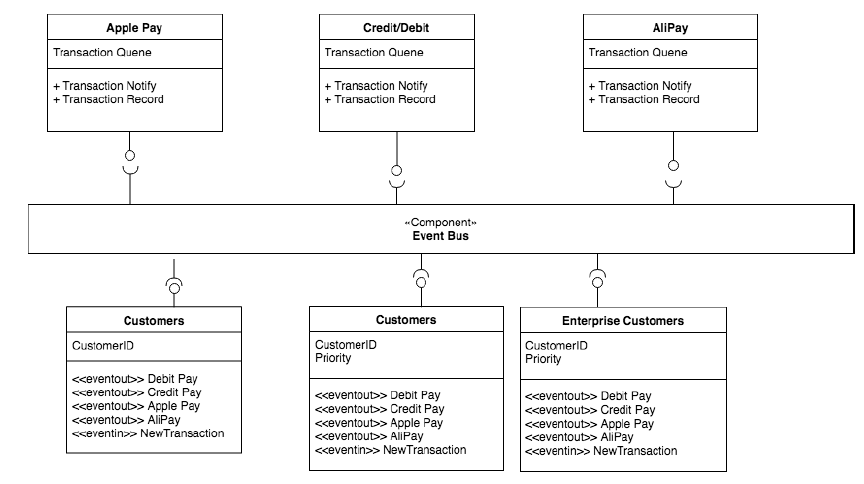
\includegraphics[width=0.4\textwidth]{./event-based}
\end{center}
